\documentclass[journal,12pt,twocolumn]{IEEEtran}

\usepackage{setspace}
\usepackage{gensymb}
\singlespacing
\usepackage[cmex10]{amsmath}

\usepackage{amsthm}

\usepackage{mathrsfs}
\usepackage{txfonts}
\usepackage{stfloats}
\usepackage{bm}
\usepackage{cite}
\usepackage{cases}
\usepackage{subfig}

\usepackage{longtable}
\usepackage{multirow}

\usepackage{enumitem}
\usepackage{mathtools}
\usepackage{steinmetz}
\usepackage{tikz}
\usepackage{circuitikz}
\usepackage{verbatim}
\usepackage{tfrupee}
\usepackage[breaklinks=true]{hyperref}
\usepackage{graphicx}
\usepackage{tkz-euclide}

\usetikzlibrary{calc,math}
\usepackage{listings}
    \usepackage{color}                                            %%
    \usepackage{array}                                            %%
    \usepackage{longtable}                                        %%
    \usepackage{calc}                                             %%
    \usepackage{multirow}                                         %%
    \usepackage{hhline}                                           %%
    \usepackage{ifthen}                                           %%
    \usepackage{lscape}     
\usepackage{multicol}
\usepackage{chngcntr}

\DeclareMathOperator*{\Res}{Res}

\renewcommand\thesection{\arabic{section}}
\renewcommand\thesubsection{\thesection.\arabic{subsection}}
\renewcommand\thesubsubsection{\thesubsection.\arabic{subsubsection}}

\renewcommand\thesectiondis{\arabic{section}}
\renewcommand\thesubsectiondis{\thesectiondis.\arabic{subsection}}
\renewcommand\thesubsubsectiondis{\thesubsectiondis.\arabic{subsubsection}}


\hyphenation{op-tical net-works semi-conduc-tor}
\def\inputGnumericTable{}                                 %%

\lstset{
%language=C,
frame=single, 
breaklines=true,
columns=fullflexible
}
\begin{document}

\newcommand{\BEQA}{\begin{eqnarray}}
\newcommand{\EEQA}{\end{eqnarray}}
\newcommand{\define}{\stackrel{\triangle}{=}}
\bibliographystyle{IEEEtran}
\raggedbottom
\setlength{\parindent}{0pt}
\providecommand{\mbf}{\mathbf}
\providecommand{\pr}[1]{\ensuremath{\Pr\left(#1\right)}}
\providecommand{\qfunc}[1]{\ensuremath{Q\left(#1\right)}}
\providecommand{\sbrak}[1]{\ensuremath{{}\left[#1\right]}}
\providecommand{\lsbrak}[1]{\ensuremath{{}\left[#1\right.}}
\providecommand{\rsbrak}[1]{\ensuremath{{}\left.#1\right]}}
\providecommand{\brak}[1]{\ensuremath{\left(#1\right)}}
\providecommand{\lbrak}[1]{\ensuremath{\left(#1\right.}}
\providecommand{\rbrak}[1]{\ensuremath{\left.#1\right)}}
\providecommand{\cbrak}[1]{\ensuremath{\left\{#1\right\}}}
\providecommand{\lcbrak}[1]{\ensuremath{\left\{#1\right.}}
\providecommand{\rcbrak}[1]{\ensuremath{\left.#1\right\}}}
\theoremstyle{remark}
\newtheorem{rem}{Remark}
\newcommand{\sgn}{\mathop{\mathrm{sgn}}}
\providecommand{\abs}[1]{\vert#1\vert}
\providecommand{\res}[1]{\Res\displaylimits_{#1}} 
\providecommand{\norm}[1]{\lVert#1\rVert}
%\providecommand{\norm}[1]{\lVert#1\rVert}
\providecommand{\mtx}[1]{\mathbf{#1}}
\providecommand{\mean}[1]{E[ #1 ]}
\providecommand{\fourier}{\overset{\mathcal{F}}{ \rightleftharpoons}}
%\providecommand{\hilbert}{\overset{\mathcal{H}}{ \rightleftharpoons}}
\providecommand{\system}{\overset{\mathcal{H}}{ \longleftrightarrow}}
	%\newcommand{\solution}[2]{\textbf{Solution:}{#1}}
\newcommand{\solution}{\noindent \textbf{Solution: }}
\newcommand{\cosec}{\,\text{cosec}\,}
\providecommand{\dec}[2]{\ensuremath{\overset{#1}{\underset{#2}{\gtrless}}}}
\newcommand{\myvec}[1]{\ensuremath{\begin{pmatrix}#1\end{pmatrix}}}
\newcommand{\mydet}[1]{\ensuremath{\begin{vmatrix}#1\end{vmatrix}}}
\numberwithin{equation}{subsection}
\makeatletter
\@addtoreset{figure}{problem}
\makeatother
\let\StandardTheFigure\thefigure
\let\vec\mathbf
\renewcommand{\thefigure}{\theproblem}
\def\putbox#1#2#3{\makebox[0in][l]{\makebox[#1][l]{}\raisebox{\baselineskip}[0in][0in]{\raisebox{#2}[0in][0in]{#3}}}}
     \def\rightbox#1{\makebox[0in][r]{#1}}
     \def\centbox#1{\makebox[0in]{#1}}
     \def\topbox#1{\raisebox{-\baselineskip}[0in][0in]{#1}}
     \def\midbox#1{\raisebox{-0.5\baselineskip}[0in][0in]{#1}}
\vspace{3cm}
\title{Assignment 9}
\author{Dishank Jain - AI20BTECH11011}
\maketitle
\newpage
\bigskip
\renewcommand{\thefigure}{\theenumi}
\renewcommand{\thetable}{\theenumi}
Download latex-tikz codes from 
%
\begin{lstlisting}
https://github.com/Dishank422/AI1103-Probability-and-random-variables/blob/main/Assignment_9/main.tex
\end{lstlisting}
\section{Problem}
(CSIR UGC NET, June 2016, Q.107)Suppose X and Y are independent and identically distributed random variables and let $Z = X + Y$. Then the distribution of $Z$ is in the same family as that of $X$ and $Y$ if X is
\begin{table}[h]
\setlength{\tabcolsep}{30pt}
    \begin{tabular}{ll}
         1) Normal  & 2) Exponential  \\
         3) Uniform & 4) Binomial
    \end{tabular}
\end{table}
\section{Solution}
\begin{enumerate}[label = \arabic*)]
    \item Let X and Y be independent and identically distributed normal random variables. Then the characteristic function of X and Y is given by
    \begin{align}
        \Phi_X(\omega) = e^{j\eta\omega - \sigma^2\omega^2/2}
    \end{align}
    The characteristic function of Z is given by
    \begin{align}
        \Phi_Z(\omega) &= \Phi_X^2(\omega)\\
                       &= e^{2j\eta\omega - \sigma^2\omega^2}
    \end{align}
    Thus Z is a normal random variable with parameters $2\eta$ and $2\sigma^2$. Thus option (1) is correct.
    \item Let X and Y be independent and identically distributed exponential random variables. Then the pdf of X and Y is given by
    \begin{align}
        f_X(x) = 
        \begin{cases}
            \lambda e^{-\lambda x} &x>0\\
            0 &otherwise
        \end{cases}
    \end{align}
    Using convolution, 
    \begin{align}
        f_z(z) = 
        \begin{cases}
            \int_0^z f_X(x)f_Y(z-x) dx &z>0\\
            0 &otherwise
        \end{cases}
    \end{align}
    Thus if $z>0$,
    \begin{align}
        f_Z(z) &= \int_0^z \lambda^2 e^{-\lambda x}e^{-\lambda(z-x)} dx\\
               &= z \lambda^2 e^{-\lambda z}
    \end{align}
    Thus Z is not an exponential random variable. Therefore option (2) is wrong.
    \item Let X and Y be independent and identically distributed uniform random variables such that X, Y $\sim$ U(a,b). Then
    \begin{align}
        f_X(x) = 
        \begin{cases}
            \dfrac{1}{b-a} &a<x<b\\
            0 &otherwise
        \end{cases}
    \end{align}
    Then, using convolution, for $2a<z<a+b$, 
    \begin{align}
        f_Z(z) &= \int_{2a}^z f_X(x)f_Y(z-x) dx\\
               &= \dfrac{z-2a}{(b-a)^2}
    \end{align}
    For $a+b<z<2b$,
    \begin{align}
        X,Y &> z - (a+b)\\
        Z &= X+Y\\
        \implies X,Y &< (b-a)\\
        \implies f_Z(z) &= \int_{z-(a+b)}^{b-a} f_X(x)f_Y(z-x)dx\\
                        &= \dfrac{2b-z}{(b-a)^2}
    \end{align}
    For $z<2a$ or $z>2b$, 
    \begin{align}
        f_Z(z) = 0
    \end{align}
    Thus Z is not a uniform random variable. Thus option (3) is wrong.
    \item Let X and Y be independent and identically distributed binomial random variables. Then the pmf of X and Y is given by
    \begin{align}
        p_X(k) = \myvec{n\\k}p^k q^{n-k}
    \end{align}
    Taking Z-transform
    \begin{align}
        p_X(z) &= \sum_{k=0}^n \myvec{n\\k} p^k q^{n-k} z^{-k}\\
               &= \left(\dfrac{p}{z}+q \right)^n
    \end{align}
    Thus
    \begin{align}
        p_Z(z) &= p_X^2(z)\\
               &= \left(\dfrac{p}{z}+q \right)^{2n}\\
               &= \sum_{k=0}^{2n} \myvec{2n\\k} p^k q^{2n-k} z^{-k}
    \end{align}
    Thus taking inverse Z-transform, 
    \begin{align}
        p_Z(k) = \myvec{2n\\k} p^k q^{2n-k}
    \end{align}
    Thus Z is a binomial random variable. Thus option (4) is correct.
\end{enumerate}
The following figures show the experimental distributions for Z in each case. The simulation length was kept one million.
\begin{figure}[!ht]
\centering
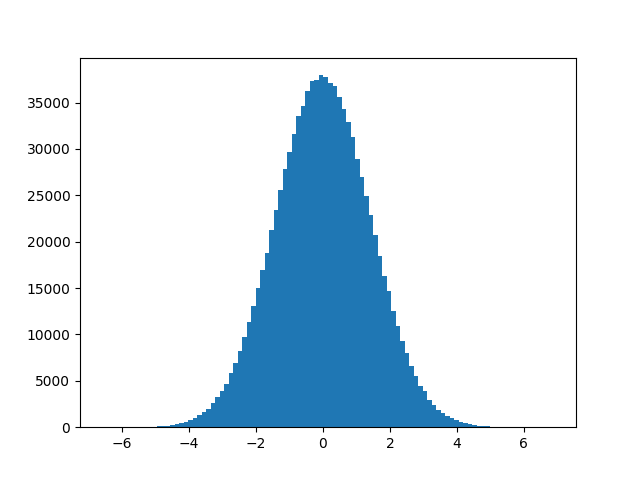
\includegraphics[width=\columnwidth]{figures/norm.png}
\caption{Z when X is standard normal}
\label{fig:normal}
\end{figure}
\begin{figure}[!ht]
\centering
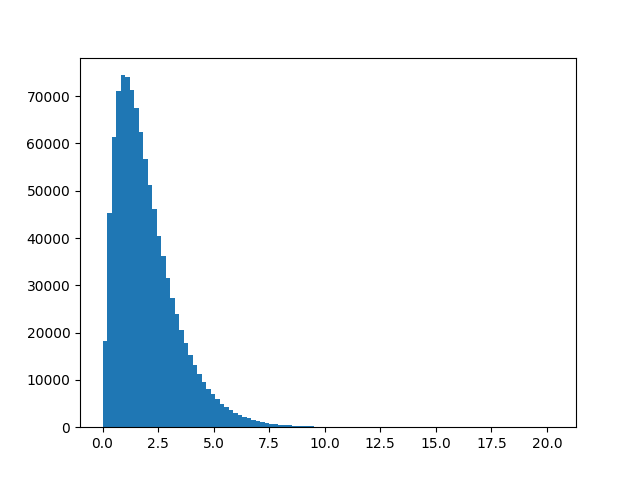
\includegraphics[width=\columnwidth]{figures/expon.png}
\caption{Z when X is exponential with $\lambda = 1$}
\label{fig:exponential}
\end{figure}
\begin{figure}[!ht]
\centering
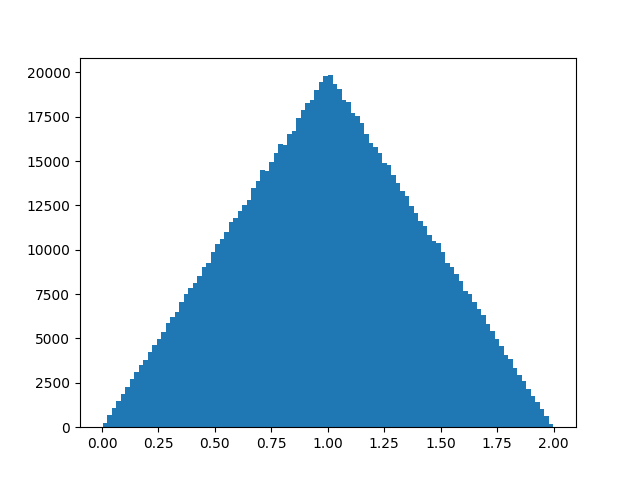
\includegraphics[width=\columnwidth]{figures/uniform.png}
\caption{Z when X $\sim$ U(0,1)}
\label{fig:uniform}
\end{figure}
\begin{figure}[!ht]
\centering
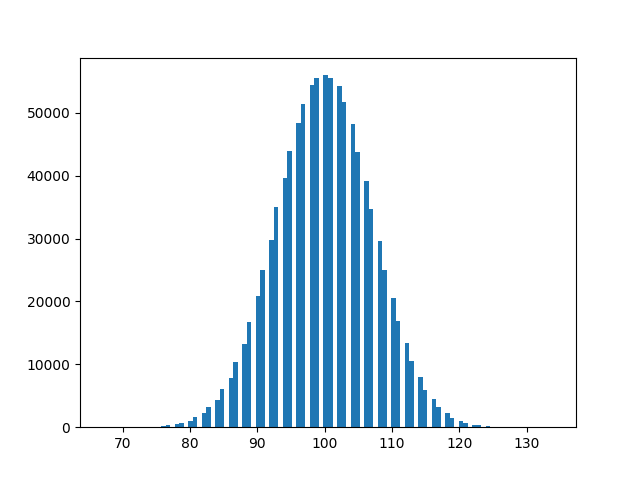
\includegraphics[width=\columnwidth]{figures/binom.png}
\caption{Z when X $\sim$ B(100,0.5)}
\label{fig:binomial}
\end{figure}
\end{document}
